
% This paper can be formatted using the peerreviewca
% (instead of conference) mode.
\documentclass[conference]{IEEEtran}


\usepackage{graphicx}  % Written by David Carlisle and Sebastian Rahtz


\usepackage{subfigure} % Written by Steven Douglas Cochran

\usepackage{url}       % Written by Donald Arseneau

\usepackage{array}
% There should be no need to do such things with IEEEtran.cls V1.6 and later.
\graphicspath{ {C:/Users/husai/OneDrive/Desktop/Mini Project/} }
% correct bad hyphenation here
\hyphenation{op-tical net-works semi-conduc-tor IEEEtran}

\providecommand{\keywords}[1]
{

	\textbf{\textit{Keywords---}} #1
}

\begin{document}
	
	% paper title
	\title{Implementation of Security System using Computer Vision and Temperature Detection}
	
	
	% author names and affiliations
	% use a multiple column layout for up to three different
	% affiliations
	\author{
		Aryan Dali\\
		\textit{Department of Electronics}\\
		\textit{and Telecommunications}\\
		\textit{Sardar Patel Institute of Technology}\\
		Mumbai, India\\
		aryan.dali@spit.ac.in
		\and
		Anand Mane\\
		\textit{Department of Electronics}\\
		\textit{and Telecommunications}\\
		\textit{Sardar Patel Institute of Technology}\\
		Mumbai, India\\
		anand\_mane@spit.ac.in
		\and
		Husain Challawala\\
		\textit{Department of Electronics}\\
		\textit{and Telecommunications}\\
		\textit{Sardar Patel Institute of Technology}\\
		Mumbai, India\\
		husain.challawala@spit.ac.in\\
		\and
		\hspace{6.3cm}Jai Damani\\
		\hspace{6.3cm}\textit{Department of Electronics}\\
		\hspace{6.3cm}\textit{and Telecommunications}\\
		\hspace{6.3cm}\textit{Sardar Patel Institute of Technology}\\
		\hspace{6.3cm}Mumbai, India\\
		\hspace{6.3cm}jai.damani@spit.ac.in\\
	}
	
	
	% make the title area
	\maketitle
	
	\begin{abstract}
		\textbf{For corporate and private groups, providing security and secure access to workplaces has long been a top priority. From keypads to fingerprint sensors, there have been advancements in the way security is delivered over the years. Even these, though, have their flaws and weaknesses. Computer Vision is a more powerful and modern technique which can be integrated into a security system for the purpose of increasing the overall level of security. This project aims to create a security system that utilizes this software as well as a temperature sensing module to enable secure, monitored and contact-less, access. The facial authentication is achieved with a help of a webcam connected to the system and a python program on which this is executed,
			after which the main control is transferred to the Arduino
			UNO Microcontroller board which tests the two incoming
			inputs and provides access based on its decision. A training model is employed which studies the given
			images of the users and detects them when entry is requested.\\}
	\end{abstract}
	
	\keywords{
		Facial Authentication, Security System, Temperature
		detection, OpenCV, Arduino UNO, Computer Vision
}
	
	%\IEEEpeerreviewmaketitle
	
	
	
	\section{Introduction}
	% no \PARstart
	In this current era, physical security breaches and risks are at an all-time high. Corporate premises ranging from residential homes to commercial
	buildings require trustworthy and high standard security
	to prevent breach and theft. Hence, designing a modified and improved security system to grant
	access only to authorized people seemed of utmost need. \\This system is considerably more
	efficient than a password-based system or a fingerprint
	system and it also eliminates all the need for any physical contact with the system which is of utmost importance in today's day and age owing to the COVID-19 pandemic. 
	The proposed system is a facial recognition security system with a temperature sensor that will be able to protect people’s
	personal spaces as well as their health. It can be deployed in protected or public areas and can serve as an effective security solution.\\ It consists of the
	following components: \\
	1. A facial recognition system implemented using python's Computer Vision. \\
	2. A temperature sensing system with the help of LM-35 temperature sensor. \\
	3. Arduino Microcontroller which oversees the logic\cite{a}.
	
	
	
	\subsection{Motivation}
	As security breaches become more common, a foolproof method is required to prevent attacks and improve the overall security of a system. Traditional methods of security, such as the use of a keypad or a fingerprint, while effective, can be easily compromised. In such cases, a stronger form of protection is required, one that recognises and authorises people based on their faces. Systems in smartphones and other devices already include a facial recognition system. Furthermore, the recent pandemic has highlighted the importance of contact-free systems and temperature checks at all entrances. This system is more scalable and can be expanded to other areas. The goal is to create a secure system that provides access through facial recognition and no contact. This system has greater complexity in implementation and thus ensures higher protection against security breaches and offers a better solution for private as well as public properties.
	
	\subsection{Literature Survey}
	The following research papers were studied for the sake of the current project-
	\begin{itemize}
		\item\textbf{Contactless Attendance Tracking using Face Recognition and Sensor based Techniques: A Pilot Study}\cite{2} \\The aim of this paper is to provide a technical review on technology which will do multiple functions like detecting faces of people with their masks on and reading their body temperature involving various techniques computer vision and deep learning using Python, OpenCV, and TensorFlow/Keras and also some sensors like Infrared Temperature Sensor.
		\item \textbf{Automatic temperature Control System using
			Arduino}\cite{3} \\Using Arduino Uno and LM35
		temperature sensor the author creates a control system based on the room temperature
		\item \textbf{Autonomous Face Detection System from Real-time Video Streaming for Ensuring the Intelligence Security System}\cite{4} \\This research paper describes an effective method for detecting and recognising facial data using OpenCV and Python, both of which are part of deep learning. A system is proposed that aids in the identification and analysis of human faces in real time which can be implemented across multiple platforms in a variety of software applications. In this paper the face detection  is done by the Haar-Cascade algorithm which is also used for designing the proposed system.
		
		\item \textbf{Convolutional Neural Network Based Smart Door Lock System}\cite{5}
		\\Due to the Covid-19 pandemic Locking systems which had means of physical touch such as bio-metric systems were banned in India. Therefore in this paper with the help of Convolutional nueral networks which recognizes a the snap of any persons face a smart locking system has been developed.
	\end{itemize}
	\subsection{Contributions}
	The primary objectives of the project are as follows-
	\begin{itemize}
		\item To develop an efficient and secure security system using modern technologies like Computer Vision. 
		\item To incorporate a contact-less temperature sensing system to determine
		the temperature thus preventing users with high risk of COVID-19 \cite{6}\cite{7}.
	\end{itemize}
	\subsection{Outline}
	\begin{itemize}
		\item The paper gives a basic idea about the design of the project, along with the
		algorithm and the implementation.
		\item The main objective is to design a face detection system
		that works with a temperature detection unit to improve security. 
		\item The use of Python and OpenCV along
		with Arduino are also discussed.
		\item Lastly, the results that were obtained at the output were discussed
	\end{itemize}
	
	\section{Body}
	\subsection{Working and algorithm}
	Designing a Facial Recognition based Security System has
	several intermittent stages. The system basically checks the users face for a match thereby sending a signal to the microprocessor (using the binary system of 1s and 0s) to allow or deny the user permission.
	After this the Arduino microprocessor has been used for
	receiving the signal from OpenCV \cite{8} and executing the
	conditional check and displaying the results of the test cases. Arduino can essentially be described as an open-source platform that is used for simulating electronics projects. It consists of an IDE (Integrated Development Environment) that can run on a computer and is used to write and upload computer code to the physical board. For the purpose of this project, an online simulation software called Proteus has been used instead of
	a physical board.
	\\If the signal received is ‘1’ and if the temperature check performed by the LM35 temperature sensor falls under the threshold range, a “Access Granted” prompt would be displayed on the LCD screen attached to the simulation circuit.
	\\Conversely, if there isn't a match in the face and the system sends a ‘0’ to the Arduino circuit, then this implies that it's an unregistered person and thus should not be granted access. And thus, an “Access Denied” prompt is generated on the screen. The LM35 is used to sense and display the temperature of the test case. After giving us the temperature, a conditional statement is constructed in the Arduino code which combines the two criteria for allowing access to a user by using an ‘if’ statement. This implies that even if the face of the person matches that with the entry in the database, if the temperature lies above a certain value (which is to say that he or she bear the risk of being COVID positive), access would not be granted to the person by the message “Temperature is too high” being
	displayed on the LCD screen.
	\\In this way a double security check is established in the system by integrating a temperature check and a facial recognition check and combining it with the circuit using the set of applications mentioned above.
	%\centering
	\begin{figure}
		\centering
		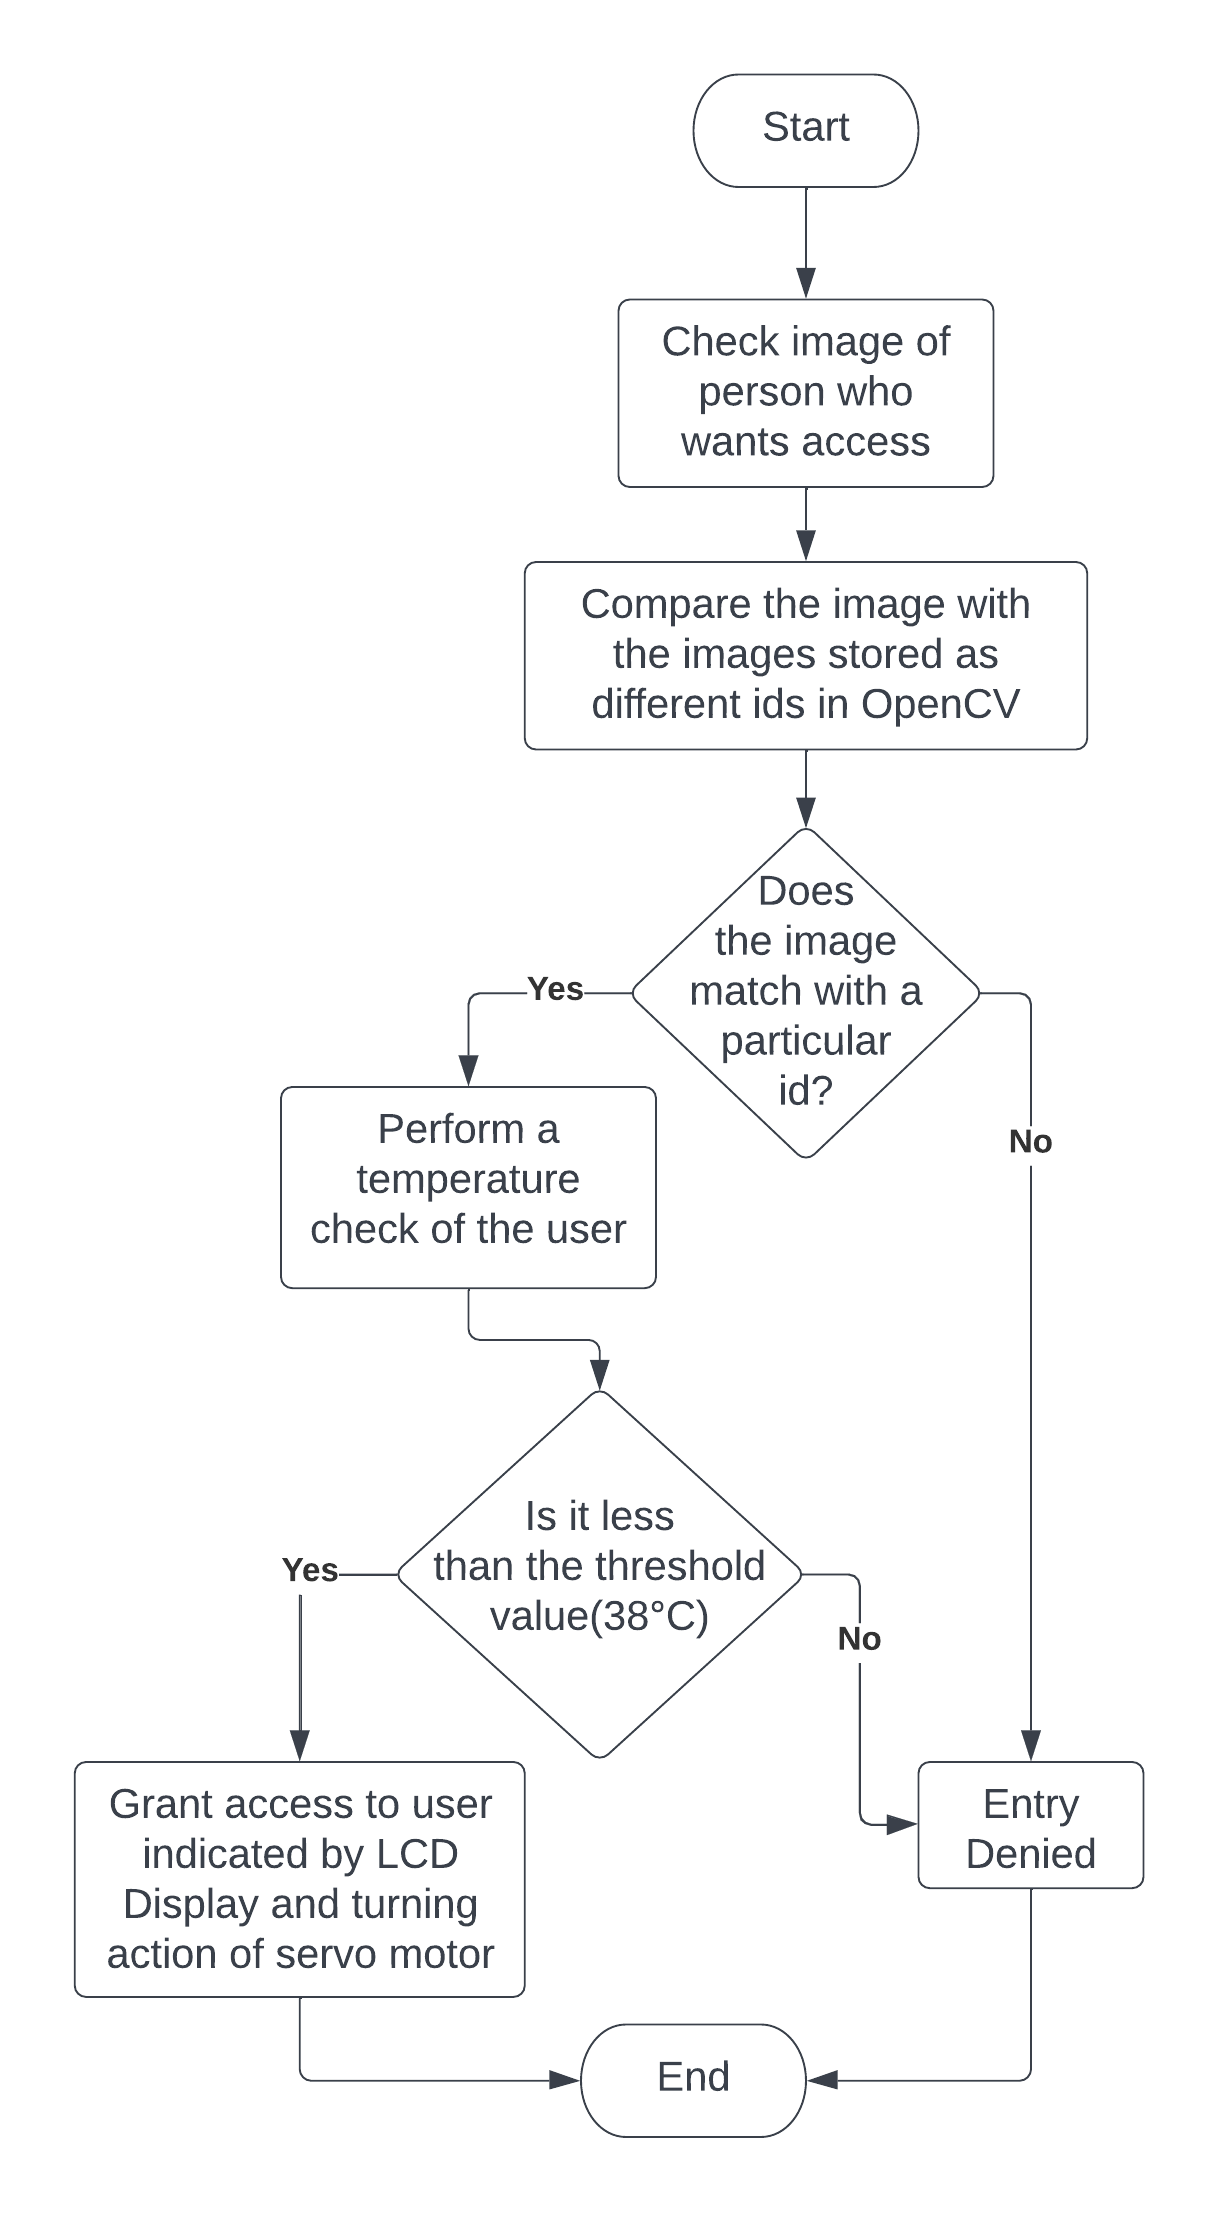
\includegraphics[width=9cm, height=15.3cm]{Flow chart.png}
		\caption{\label{fig:caption}Flow Chart}
	\end{figure}
	\subsection{Simulation}
	The system is ready for simulation after the circuit has been designed and the necessary software applications have been used. The system is first completely virtualized for testing and debugging. Python's Haar-Cascade algorithm is employed for analyzing and detecting the facial data. It is an object detection algorithm that employs edge and line detection features. The facial recognition data is sent to the Arduino board by the Python script. The Arduino takes this input and further decides whether to grant or deny access to the current user based on the temperature sensor input, which is provided by the subject. Depending on whether the system is run as a simulation or through hardware, two additional software applications may be required. Proteus Simulation Software is used to build the circuit during simulation or system testing. The system is completed by adding all of the required components and programming the microcontroller according to the set logic executed via code.
	A Virtual Serial Port Emulator is also used in conjunction with this. It is a tool for emulating serial ports for communication purposes \cite{9}. It enables the connection of the computer's various ports thus allowing Python and the microcontroller to communicate and exchange data. During hardware implementation, this is accomplished by manually connecting the Arduino to a computer and selecting the appropriate port to send data. The circuit consists of the microcontroller, LCD Screen, Servo Motor, LM-35 and a few LEDs. \\
	The LCD and LEDs are used as visual indicators for granting or denying access\cite{10}. A servo motor is used to emulate the opening and closing of an automatic door to allow entry. It rotates back to its original position within a few seconds. 
	\begin{figure}
		\centering
		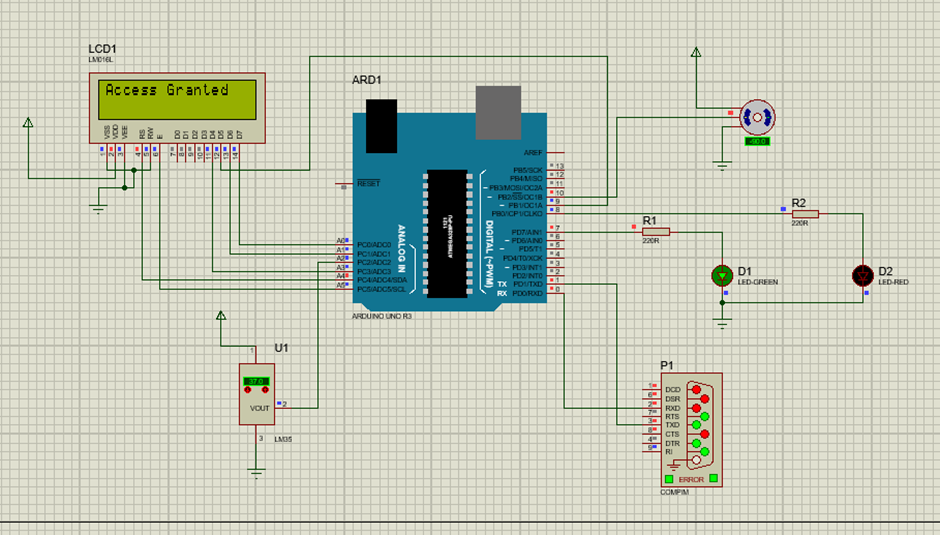
\includegraphics[width=8.5cm, height=5cm]{ProtC1.png}
		\caption{\label{fig:The-caption}Case 1: Access Granted}
	\end{figure}
	\begin{figure}
		\centering
		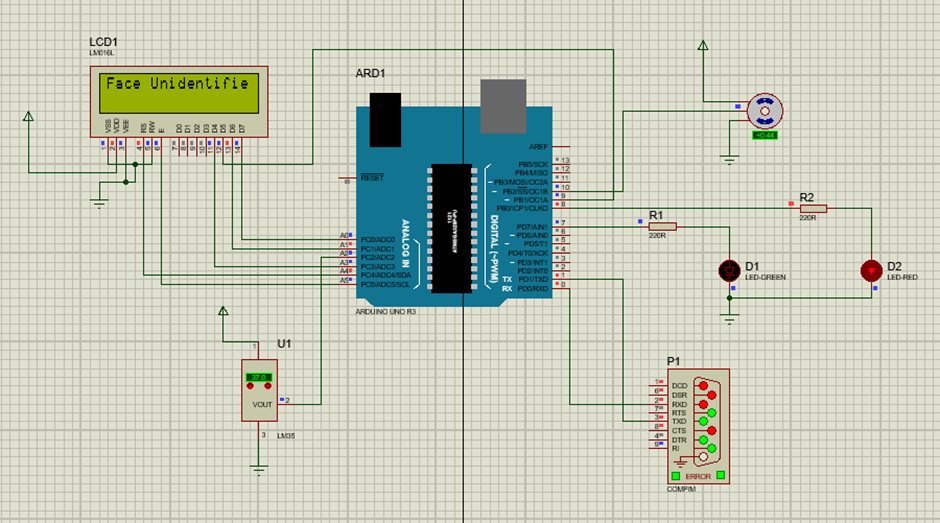
\includegraphics[width=8.5cm, height=5cm]{ProtC2.png}
		\caption{\label{fig:The-caption}Case 2: Access Denied since face is unidentified}
	\end{figure}
	\begin{figure}
		\centering	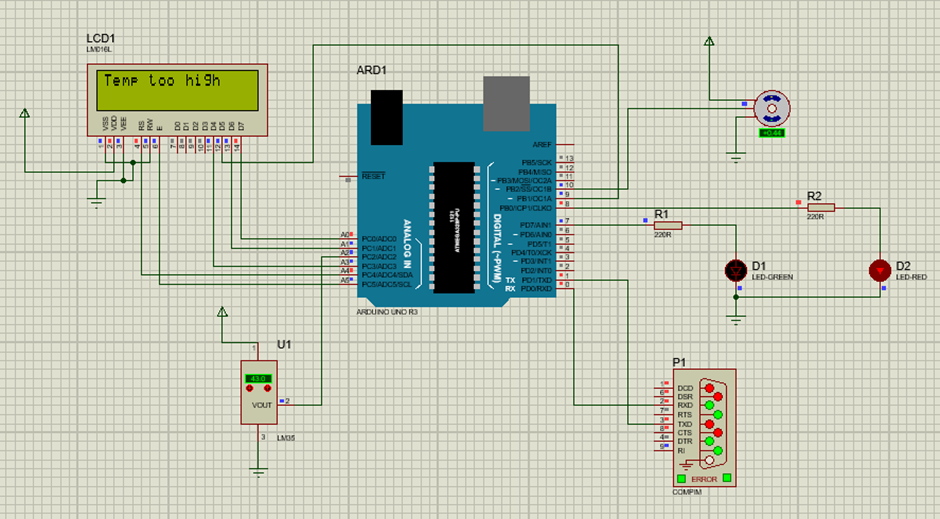
\includegraphics[width=8.5cm, height=5cm]{ProtC3.png}
		\caption{\label{fig:The-caption}Case 3: Access Denied since temperature is too high}
	\end{figure}
	\subsection{Methodology}
	\subsubsection{Facial Recognition System}
	The facial recognition system was made using OpenCV library installed in Python wherein the following steps take place \cite{11}.
	\begin{itemize}
		\item Datasets are created based on the data collected. Each dataset is assigned a unique identifier.
		\item With the gathered data set the recognizer is trained using the Haar Cascade machine learning-based approach where a lot of positive and negative images are used to train the classifier.
		\item To train on, the algorithm is given a large number of positive images with faces and a large number of negative images with no faces.
		\item Haar cascade employs the cascading window to compute features in each window and classify whether it is an object.
		\item Now that the recognizer is trained if the if there is
		an input of a face to the system then the system
		will compare it to the dataset.
		\item If there is a match with any id in the dataset with the recognize, the face will be recognised and the user is prompted towards the next phase.\\
	\end{itemize}
	\subsubsection{Temperature Sensing System}
	The temperature sensing
	stem with the help of LM-35 temperature sensor functions
	in the following steps \cite{12}.
	\begin{itemize}
		\item The LM-35 temperature sensor senses the
		temperature of the user.
		\item The analogue temperature voltage is transformed to a digital value and delivered to the Arduino UNO for processing.
		\item The Arduino compares the temperature to the set
		threshold temperature (100 F or 38 C).
		\item If the temperature of the user is less than the
		threshold temperature only then will it be presumed safe to
		grant access.\\
	\end{itemize}
	\subsubsection{Servo Motor}
	The Servo Motor utilised is a regular motor that simulates a precise and regulated circular rotation in a system \cite{13}. It is used as mentioned below:
	\begin{itemize}
		\item Only when both of the needed requirements are met, namely a match in the facial scan and a body temperature below a specified threshold, is the servo motor engaged and ordered to rotate precisely 90 degrees.
		\item This rotation is used to imitate the unlocking of the door, allowing the user to gain entrance.\\\\
	\end{itemize}
	
	\begin{figure}
		\centering
		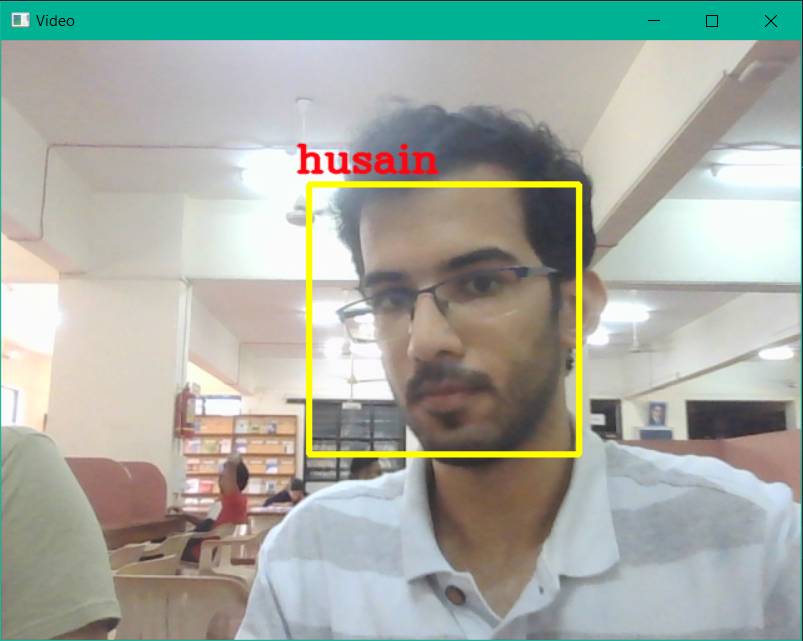
\includegraphics[width=8.5cm, height=7cm]{Husain.png}
		\caption{\label{fig:The-caption}Case 1: Identified Person 1}
	\end{figure}
	\begin{figure}
		\centering
		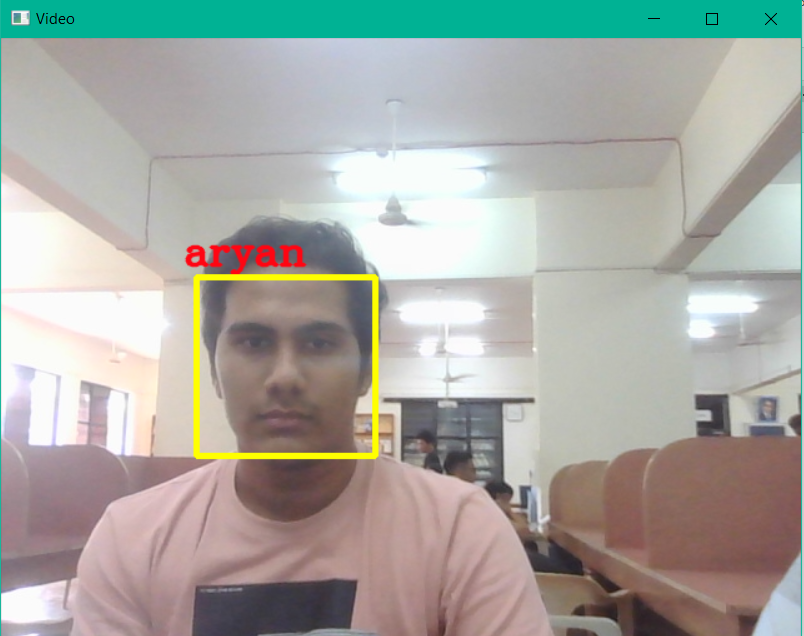
\includegraphics[width=8.5cm, height=7cm]{Aryan.png}
		\caption{\label{fig:The-caption}Case 2: Identified Person 2}
	\end{figure}
	\begin{figure}
		\centering
		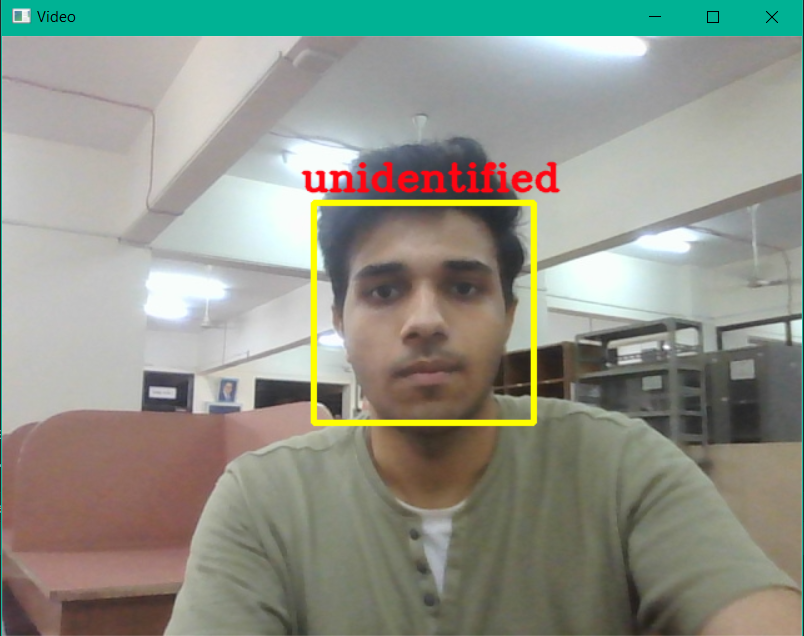
\includegraphics[width=8.5cm, height=7cm]{Un.png}
		\caption{\label{fig:The-caption}Case 3: Unidentified Person}
	\end{figure}
	\section{Results}
	Since OpenCV is used for the system, which requires a dataset of images as training models \cite{14}, 100 images of 3 people were added to the directory. These were analyzed by the algorithm as a set of coordinates and the images were compared with the faces on the webcam. For test purposes, 2 of the faces were detected since they matched with the data in the directory and one was detected as unidentified, thus posing as a security threat.\\
	The values of accuracy are an approximation after running various tests. The loss in accuracy comes primarily from the algorithm used via the face recognition system. Its accuracy can be improved by using a camera with better resolution, deploying the system in a well-lit place, altering the algorithm used or using a better one, and providing a greater set of data to train the model to improve detection. The following table shown below depicts the accuracy of the system observed under various lighting conditions- Ideal, Normal and Dim scenarios. The tests were run 20 times for each condition to correctly estimate the efficiency of this system. \\
	
	\begin{center}
		\begin{center}
			\caption{Accuracy Table:}
			\label{tab:}
			\begin{tabular}{l|c|r} % <-- Alignments: 1st column left, 2nd middle and 3rd right, with vertical lines in between
				\textbf{Lighting Conditions} & \textbf{Number of Attempts} & \textbf{Accuracy}\\
				\hline
				Ideal Lighting & 20 & 95\% \\
				Normal Lighting & 20 & 85\% \\
				Dim Lighting & 20 & 60\% \\
			\end{tabular}
		\end{center}
		\label{tab:caption}
	\end{center}
	
	\hfill
	\section{Conclusion and Future Scope}
	The primary objective of this project was to provide a security system that eliminated the use of passwords (which may be forgotten and are relatively unsafe and can also be compromised) and fingerprints that can act as a means to spread diseases which is highly unsuitable given the current COVID-19 pandemic situation. The facial recognition system proposed is much more accurate as compared to a fingerprint-based system and since it is combined with a temperature sensor, it provides an additional check for body temperature which is now a mandatory security parameter in malls and offices worldwide. It also provides for a cost-effective and user-friendly design.\\
	We have used several platforms for the system that perform their specific tasks. The main component was the OpenCV library, which was used to detect and recognise the faces of people. The next main component is the micro controller, which performs the conditional check and authorises the entry of the person. The entire system is simulated on Proteus for the sake of this project. 
	
	The project's future scope would include implementing the system with physical components and integrating it with voice recognition-based software to boost security and complexity while reducing security breaches\cite{15}. It might also be possible to eliminate the requirement of a temperature sensor entirely by introducing a Machine Learning model that can detect approximate temperature based on a colour-temperature correlation approach \cite{16}.
	
	% use section* for acknowledgement
	\section*{Acknowledgment}
	% optional entry into table of contents (if used)
	\addcontentsline{toc}{section}{Acknowledgment}
	Taking this opportunity to express our sincere
	thanks to our guide Prof Anand Mane,
	Professor of Electronics and Telecommunication
	Engineering, S.P.I.T., Mumbai, for providing the
	technical guidelines and the suggestions regarding line the
	of this work. Also expressing gratitude
	towards his constant encouragement, support and
	guidance throughout the development of the project.
	
	\begin{thebibliography}{1}
		
		\bibitem{a}
		Louis, Leo. (2018). Working Principle of Arduino and Using it as a Tool for Study and Research. International Journal of Control, Automation, Communication and Systems. 1. 10.5121/ijcacs.2016.1203.
		
		\bibitem{2}
		S. Sasikala, B. B. Abeshek, T. Keerthivasan, C. V. Kavi Prakash, K. Rishi and S. Arun Kumar, "Contactless Attendance Tracking using Face Recognition and Sensor based Techniques: A Pilot Study," 2021 International Conference on Advancements in Electrical, Electronics, Communication, Computing and Automation (ICAECA), 2021, pp. 1-7, doi: 10.1109/ICAECA52838.2021.9675768.
		
		\bibitem{3}
		Raju, Srujan \& Sinha, Professor G. (2020). Automatic Temperature Control System Using Arduino. Advances in Intelligent Systems and Computing. 1090. 219-226. 10.1007/978-981-15-1480-7\_18. 
		
		\bibitem{4} 
		M. A. Hoque, T. Islam, T. Ahmed and A. Amin, "Autonomous Face Detection System from Real-time Video Streaming for Ensuring the Intelligence Security System," 2020 6th International Conference on Advanced Computing and Communication Systems (ICACCS), 2020, pp. 261-265, doi: 10.1109/ICACCS48705.2020.9074260.
		
		\bibitem{5}
		R. Mishra, A. Ransingh, M. K. Behera and S. Chakravarty, "Convolutional Neural Network Based Smart Door Lock System," 2020 IEEE India Council International Subsections Conference (INDISCON), 2020, pp. 151-156, doi: 10.1109/INDISCON50162.2020.00041.
		
		\bibitem{6}
		S. Dash, S. Chakravarty, S. N. Mohanty, C. R. Pattanaik, and S. Jain, “A deep learning method to forecast COVID-19 outbreak,” New Gener. Comput., vol. 39, no. 3–4, pp. 515–539, 2021.
		
		\bibitem{7}
		N. Mahesh, G. S. Deepak Prasath, E. Divyadharshini and V. Gokul, "Implementation of Covid-19 Health Monitoring System," 2022 International Conference on Electronics and Renewable Systems (ICEARS), 2022, pp. 1516-1520, doi: 10.1109/ICEARS53579.2022.9752163.
		
		\bibitem{8}
		A. Arunraja, C. A. Prasath, D. A. G and H. K S, "Design of Open CV, EAR Algorithm and DLib Library for Smart Home Controller," 2022 6th International Conference on Computing Methodologies and Communication (ICCMC), 2022, pp. 1501-1504, doi: 10.1109/ICCMC53470.2022.9754017.
		
		\bibitem{9}
		“DB9 changer datasheet PDF,” DB9 Datasheet | ETC - Datasheetspdf.com. [Online]. Available: https://datasheetspdf.com/datasheet/DB9.html. [Accessed: 02-Apr-2022].
		
		\bibitem{10}
		“16x2 LCD display module,” Circuit Digest, 17-Jul-2018. [Online]. Available: https://circuitdigest.com/article/16x2-lcd-display-module-pinout-datasheet. [Accessed: 02-Apr-2022].
		
		\bibitem{11}
		Mahamkali, Naveenkumar \& Ayyasamy, Vadivel. (2015). OpenCV for Computer Vision Applications. 
		
		
		
		\bibitem{12} 
		“Temperature measurement using LM35 and AVR microcontroller,” MaxPhi, 16-Sep-2017. [Online]. Available: https://www.maxphi.com/temperature-measurement-using-lm35-and-avr-microcontroller. [Accessed: 02-Apr-2022]. 
		
		\bibitem{13}
		“Servo Motor SG-90,” Components101. [Online]. Available: https://components101.com/motors/servo-motor-basics-pinout-datasheet. [Accessed: 02-Apr-2022].
		
		\bibitem{14}
		Tejashree Dhawle, Urvashi Ukey \& Rakshandha Choudante. Face Detection and Recognition using OpenCV and Python. International Research Journal of Engineering and Technology (IRJET), Volume: 07 Issue: 10 | Oct 2020
		
		\bibitem{15}
		A. D and S. P, "Face Recognition Authenticated Voice Assistant System for the disabled," 2021 Second International Conference on Electronics and Sustainable Communication Systems (ICESC), 2021, pp. 1220-1226, doi: 10.1109/ICESC51422.2021.9533017.
		
		\bibitem{16}
		G. Agrawal, R. Mishra, A. Ransingh and S. Chakravarty, "Flame Temperature Prediction Using Machine Learning Model," 2020 IEEE India Council International Subsections Conference (INDISCON), 2020, pp. 157-162, doi: 10.1109/INDISCON50162.2020.00042.
		
		
		
		
		
		
		
		
		
	\end{thebibliography}
\end{document}











